% !TeX encoding = UTF-8
\documentclass[12pt,A4paper,titlepage]{article}
\usepackage[spanish]{babel}
\usepackage[utf8]{inputenc} %Este paquete permite poner acentos directamente y ees
\usepackage[T1]{fontenc}
\usepackage{amsmath}
\usepackage{graphicx}%[pdftex]
\usepackage{graphicx, wrapfig}
\usepackage{fancyhdr}
\usepackage{anysize}
\usepackage{verbatim}
\usepackage[dvips,final]{epsfig}
\usepackage{epstopdf}
\usepackage{colortbl}
\usepackage{listings}
\usepackage{float}
\usepackage{color}
\marginsize{2.5cm}{2.5cm}{2.5cm}{2.5cm}
\usepackage{fancyhdr}
\pagestyle{fancy}
\fancyhf{}
\fancyhead[LO]{Arquitectura de Computadoras}
\fancyfoot[LE,RO]{\thepage}
\fancyfoot[LO]{Aagaard Martín - Navarro Matias}
\renewcommand{\footrulewidth}{0.4pt}


%\graphicspath{{figuras/}}

%defiino un estilo de ingreso de codigo
\definecolor{codegreen}{rgb}{0,0.6,0}
\definecolor{codegray}{rgb}{0.5,0.5,0.5}
\definecolor{codepurple}{rgb}{0.58,0,0.82}
\definecolor{backcolour}{rgb}{0.95,0.95,0.92}
 
\lstdefinestyle{mystyle}{
    backgroundcolor=\color{backcolour},   
    commentstyle=\color{codegreen},
    keywordstyle=\color{magenta},
    numberstyle=\tiny\color{codegray},
    stringstyle=\color{codepurple},
    basicstyle=\footnotesize,
    breakatwhitespace=false,         
    breaklines=true,                 
    captionpos=b,                    
    keepspaces=true,                 
    numbers=left,                    
    numbersep=5pt,                  
    showspaces=false,                
    showstringspaces=false,
    showtabs=false,                  
    tabsize=2
}
\lstset{style=mystyle}
\setlength{\parindent}{1cm}
\setlength{\parskip}{\baselineskip} 

\begin{document}
\renewcommand{\tablename}{Tabla}
\large

\title{Arquitectura de Computadoras \\
\large Trabajo Páctico Nº3 - BIP}
\author{Aagaard Martin - Navarro Matias
\bigskip
\bigskip}

\date{Universidad Nacional de Córdoba \\ 20 de noviembre de 2019}

\begin{titlepage}
\center


\begin{figure}[h]
    \centering
    
\includegraphics[scale=0.8]{figure/logos-fcefyn-y-unc.png}
    \label{fig:unc-logo}
\end{figure}

{\let\newpage\relax\maketitle}
\center
\end{titlepage}

\maketitle % Compila la carátula
\tableofcontents % Arma el índice
\newpage

\section{Introducción}
En el siguiente trabajo se realizó la implementación en Verilog de un procesador BIP I. Se desarrolló para la placa Basys 3, utilizando el software Vivado 2018.2. El procesador permite la ejecución de instrucciones simples en un ciclo. Es posible visualizar el resultado de las instrucciones ejecutadas desde la placa: ciclos de clock empleados, y el resultado final en un registro acumulador.

Las operaciones que se pueden realizar son:

\begin{figure} [H]
    \centering
    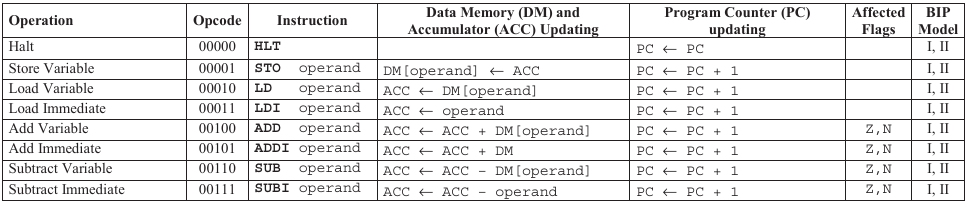
\includegraphics[width=\textwidth]{figure/BIP-instruc.png}
    \caption{\textit{Instrucciones del BIP I}}
    \label{fig:BIP-instruc}
\end{figure}

\section{Desarrollo}
Se definió un módulo Top, que contiene: 
\begin{itemize}
    \item Módulo CPU
    \item Módulo RAM de Instrucciones
    \item Módulo RAM de Datos
\end{itemize}

\subsection{CPU}
El módulo CPU contiene una implementación del procesador BIP I en Verilog. Se descompuso en los siguientes bloques funcionales: control y datapath.
\begin{figure} [H]
    \centering
    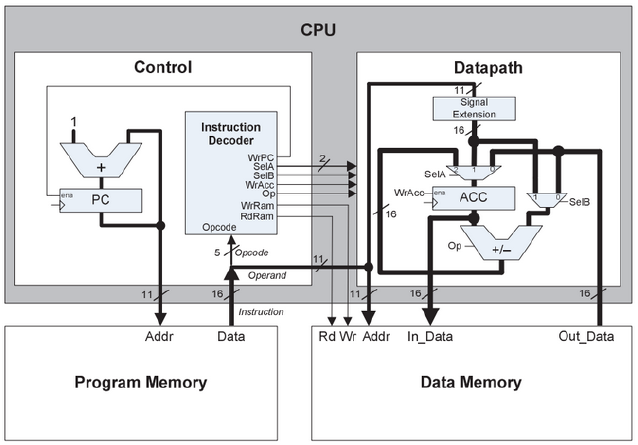
\includegraphics[scale=0.85]{figure/DB-BIP-I.png}
    \caption{\textit{Diagrama de bloques del procesador BIP I}}
    \label{fig:DB-BIP-I}
\end{figure}

\subsubsection{Control}
El bloque de control del BIP se encarga de obtener la siguiente instrucción de la memoria de programa, la posición buscada indicada por el valor del registro PC. Además, posee un circuito combinacional que controla mediante diversas señales, el comportamiento del bloque de datapath, aquí se controlará exactamente que instrucción se realiza dependiendo las condiciones que se habilitan en el mismo. El único elemento controlado por el clock en este bloque es el registro PC.

\textbf{Instruction Decoder} \\
Este bloque habilita todas las señales necesarias para que se realiza la operación leída en el ciclo de clock. La parte llamada \textit{opcode} (los 5 bits mas significativos) del la instrucción leída de la memoria de programa entran a este bloque y, dependiendo de esto, el circuito combinacional modifica la salida. Las señales salientes son cables conectados al bloque datapath y a la memoria de datos (señales de escritura y lectura).

\subsubsection{Datapath}
Este bloque maneja el cálculo del resultado de la instrucción en curso. Trabaja accediendo a la memoria de datos según sea necesario, para almacenar un resultado, o leerlo y utilizarlo en una operación. Posee un único registro acumulador, una simple unidad aritmética, que permite realizar sumas y restas, y diversos multiplexores para seleccionar el dato con el que operar. Las señales de control mencionadas anteriormente se utilizan para controlar estos multiplexores, la escritura del registro acumulador, y el comportamiento de la memoria de datos (lectura o escritura).

\subsection{RAM de Instrucciones y de Datos} \label{ram-de-instrucciones-y-de-datos}
Estos bloques se generaron mediante los templates que provee el entorno de desarrollo. Consisten en memorias de 16 bits, 2048 registros para las instrucciones y 1024 registros para los datos.
La memoria de instrucciones fue inicializada con un archivo \textit{.mem}, que contiene las instrucciones en binario utilizadas para probar el funcionamiento del BIP.

\begin{figure} [H]
    \centering
    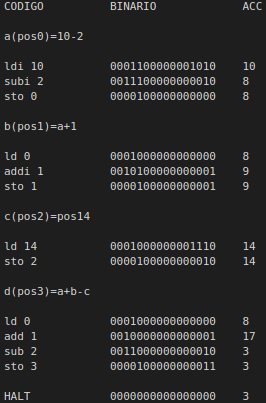
\includegraphics{figure/program_memory.png}
    \caption{\textit{Programa cargado en la memoria de programa}}
    \label{fig:program_memory.txt}
\end{figure}

Un punto importante a destacar es el empleo del modo \textbf{Low Latency} para la memoria de datos. Esto fue necesario ya que, como las instrucciones deben completarse en un ciclo, se encontraron escenarios en los que esto no era posible, por ejemplo, si una instrucción solicita sumar el valor del acumulador con el guardado en una posición de la memoria de datos, la secuencia de operaciones a realizar es:
\begin{enumerate}
    \item Leer el opcode de la memoria de programa.
    \item Interpretarla y emitir las señales de control.
    \item Leer el valor en memoria de datos a sumar.
    \item Sumar el acumulador con el valor leído.
    \item Guardar el resultado donde corresponda.
\end{enumerate}

Todo el proceso debe realizarse en un ciclo, por requerimiento de diseño del procesador. Pero si se trabaja con un solo flanco no es posible, por lo que las operaciones con la memoria de programa se realizan en un flanco, y las de datos en el otro. Esto permite cumplir con los requisitos planteados sin comprometer el rendimiento del sistema.

\subsection{ALU}
El módulo ALU es el desarrollado en el primer práctico. Es puramente combinacional, con dos entradas para operandos, una entrada para el operador y una salida con el resultado de la operación.

\begin{figure}[h] 
	\centering
	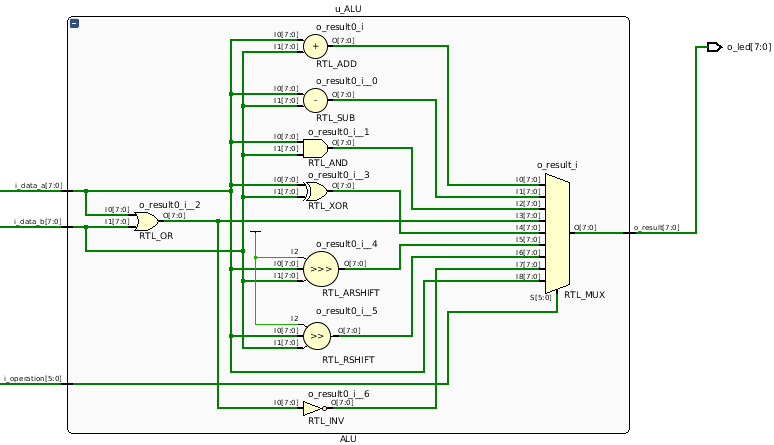
\includegraphics[scale=0.6]{figure/rtl-alu.png}
	\caption{\textit{Estructura RTL del módulo ALU obtenida de la herramienta Verilog}}
\end{figure}


\section{Test Bench}
Se realizaron las siguientes simulaciones para comprobar el correcto funcionamiento de cada uno de los bloques del sistema.

\subsection{CPU}
Permite verificar el correcto funcionamiento del procesador BIP en su totalidad, al interactuar con ambos bloques de memoria. Brinda información sobre el resultado en el acumulador, los valores escritos en memoria de datos, y el flujo de ejecución en general.

En la captura de pantalla \ref{fig:tb-CPU} pueden verse los valores de las distintas señales de control luego de interpretadas diversas instrucciones.

\begin{figure}[h] 
	\centering
	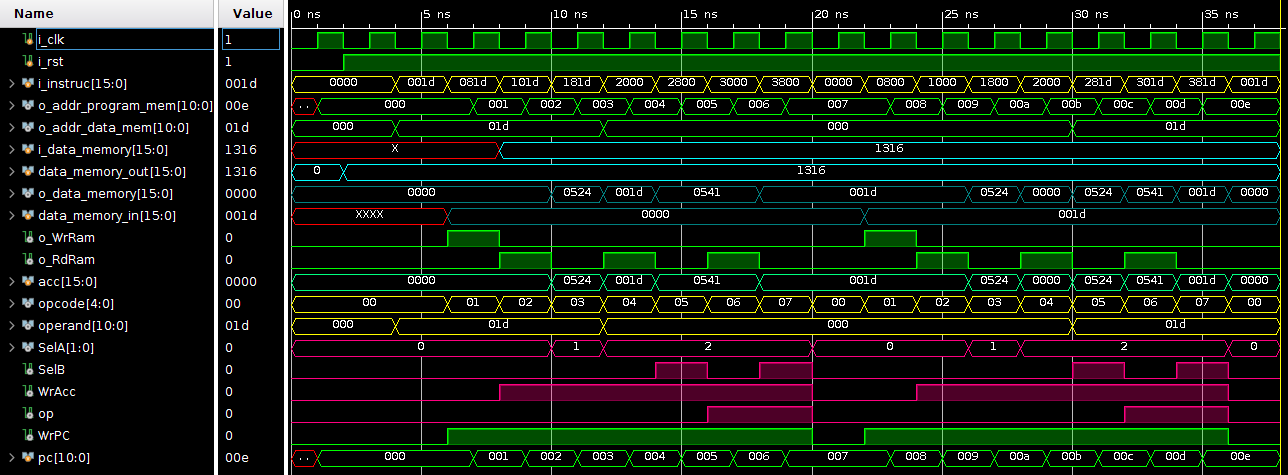
\includegraphics[width=\textwidth]{figure/tb-CPU.png}
	\caption{\textit{Resultado del test bench del CPU}}
    \label{fig:tb-CPU}
\end{figure}

\subsection{Bloque de Control}
Comprueba el correcto funcionamiento del bloque de control, dado un conjunto de instrucciones en la memoria de programa. Permite visualizar la salida del circuito combinacional que maneja el bloque de datapath.

\subsection{Instruction Decoder}
Comprueba el correcto funcionamiento del bloque de decodificación de instrucciones, dado un \textit{opcode} (parte de la instrucción). Permite visualizar la salida del circuito combinacional, observando los valores de las señales de control.

\subsection{Datapath}
Se testeó que el módulo se comporte adecuadamente frente a señales de control determinadas que representan una operación o instrucción.

\subsection{RAM de Instrucciones y de Datos}
Se comprobó la carga de datos, que sean síncronas con el clock y que el flanco en el cual devuelven el dato solicitado sea el correcto.

\subsection{Top BIP\_I}
Comprueba el correcto funcionamiento del bloque que engloba y conecta todos los otros bloques. Permite visualizar algunos registros claves (PC y ACC) durante la ejecución del programa previamente cargado a la memoria de programa (ver sección \ref{ram-de-instrucciones-y-de-datos}).
\begin{figure}[h] 
	\centering
	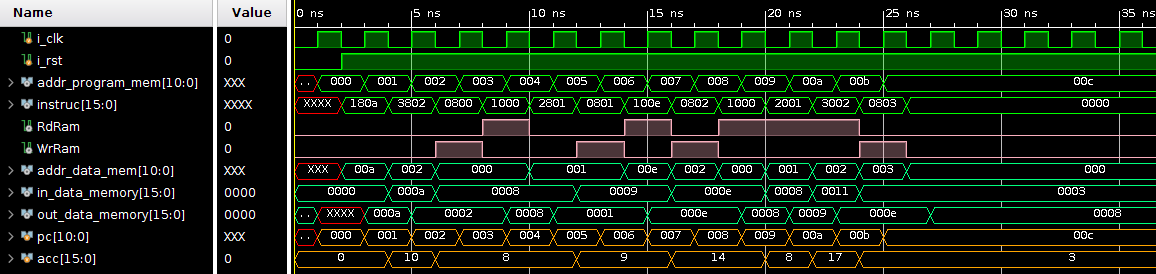
\includegraphics[width=\textwidth]{figure/tb-topBIP.png}
	\caption{\textit{Resultado del test bench del Top BIP\_I}}
    \label{fig:tb-topBI}
\end{figure}


\newpage
\section{Conclusión}
Una vez terminado el práctico, a través de la herramienta Vivado se
obtuvieron las especificaciones en la utilización de los recursos de la FPGA y en la potencia que consume dicho circuito instanciado.

Además, en este práctico se afianzaron los conceptos en cuanto al lenguaje de descripción de hardware Verilog, aprendimos sobre la utilización de bloques de memoria y sobre como utilizar un modulo de control.

\begin{figure}[H] 
	\centering
	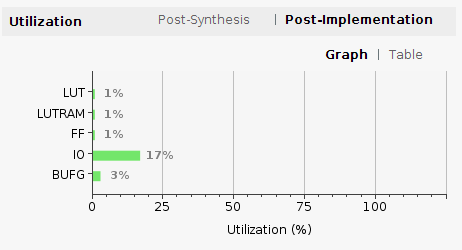
\includegraphics[scale=0.7]{figure/utilizacion.png}
	\caption{\textit{Utilización de la FPGA}}
\end{figure}

\end{document}

